% Sizes
\pgfmathsetmacro{\cardwidth}{6.3}
\pgfmathsetmacro{\cardheight}{8.8}

\pgfmathsetmacro{\verticalspacing}{0.4}
\pgfmathsetmacro{\horizontalspacing}{0.4}

\pgfmathsetmacro{\abilitywidth}{\cardwidth-2*\horizontalspacing}
\pgfmathsetmacro{\fullabilityheight}{\cardheight-2*\verticalspacing}
\pgfmathsetmacro{\halfabilityheight}{0.5*(\cardheight-3*\verticalspacing)}
\pgfmathsetmacro{\abilitybannerwidth}{1}
\pgfmathsetmacro{\abilityiconsize}{0.5}
\pgfmathsetmacro{\abilitytextwidth}{\abilitywidth-\abilitybannerwidth-0.4}

% Shapes
\def\shapeCard{(0,0) rectangle (\cardwidth,\cardheight)}

\tikzset{
	cardcorners/.style={
		rounded corners=0.2cm
	}
}
\tikzset{
	smallcardcorners/.style={
		rounded corners=0.1cm
	}
}

% Commands
\newcommand{\cardborder}{
	\draw[lightgray,cardcorners] \shapeCard;
}


\pgfmathsetmacro{\costcirclesize}{0.5}
\newcommand{\cardcost}[1]{
	\filldraw[red,fill=white!85!red] (\cardwidth-\costcirclesize-\horizontalspacing, \cardheight-\costcirclesize-\verticalspacing) circle (\costcirclesize cm);
	\node[text width=1.5cm] at (\cardwidth-\costcirclesize-\horizontalspacing, \cardheight-\costcirclesize-\verticalspacing+0.5*\costcirclesize) {
		\begin{center}
			\Large \textbf #1
		\end{center}
	};
}

\newcommand{\triggeredSelfAbility}{
	\node at (0.2*\cardwidth, 0.7*\cardheight) {
		
\includegraphics[width=1cm]{icons/self_player_grey.png}
	};
	\draw (0.5*\cardwidth-0.5, 0.5*\cardheight) circle (0.1);
	\draw (0.5*\cardwidth+0.5, 0.5*\cardheight) circle (0.1);
}
\newcommand{\triggeredOtherAbility}{
	\node at (0.2*\cardwidth, 0.7*\cardheight) {
		
\includegraphics[width=1cm]{icons/any_player_grey.png}
	};
	\draw (0.5*\cardwidth-0.5, 0.5*\cardheight) circle (0.1);
	\draw (0.5*\cardwidth+0.5, 0.5*\cardheight) circle (0.1);
}

\newcommand{\activatedAbility}{
	\node at (0.5*\cardwidth, 0.7*\cardheight) {
		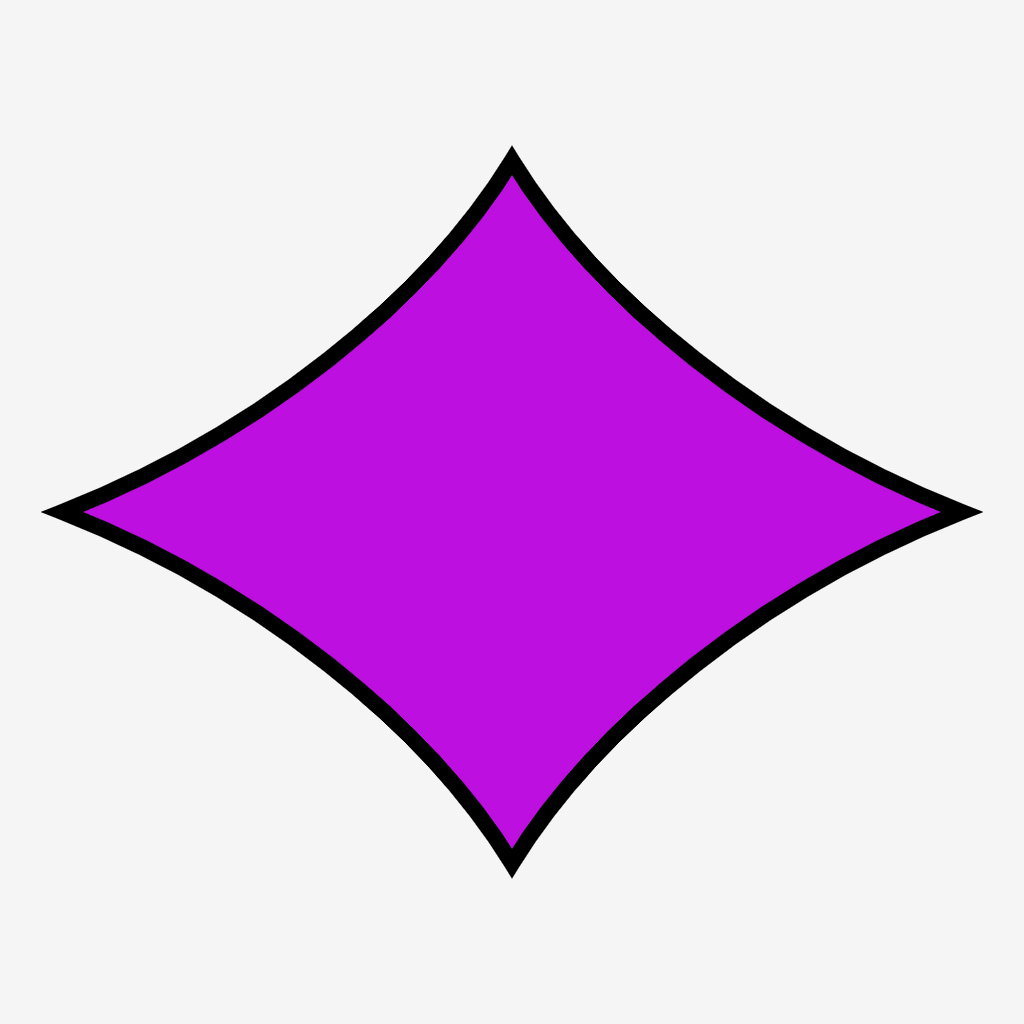
\includegraphics[width=1.5cm,height=3cm]{icons/activation_diamond_purple_189-16-224.png}
	};
	\node at (0.5*\cardwidth, 0.5*\cardheight) {
		
\includegraphics[width=1cm]{icons/down_arrow_gray.png}
	};	
}

\newcommand{\activationCost}[1]{
	\filldraw[red,fill=white!85!red] (0.5*\cardwidth+\costcirclesize+2*\horizontalspacing, 0.5*\cardheight) circle (\costcirclesize cm);
	\node[text width=1.5cm] at (0.5*\cardwidth+\costcirclesize+2*\horizontalspacing, 0.5*\cardheight+0.5*\costcirclesize) {
		\begin{center}
			\Large \textbf #1
		\end{center}
	};
}

\newcommand{\topPlaceTile}[2]{
	\node[flathexa,fill=#1] at (0.5*\cardwidth, 0.7*\cardheight-0.5*\hexSize) {
		\includegraphics[width=\hexIconSize cm]{#2}
	};
}
\newcommand{\topDrawCard}{
	\node at (0.5*\cardwidth, 0.7*\cardheight) {
		
\includegraphics[width=2cm]{icons/card_draw.png}
	};
}
\newcommand{\topTileFlip}{
	\draw[black,smallcardcorners,fill=white] (0.5*\cardwidth-0.6,0.7*\cardheight-0.6) rectangle (0.5*\cardwidth+0.6,0.7*\cardheight+0.6);
	\node at (0.5*\cardwidth+0.4, 0.7*\cardheight-0.2) {
		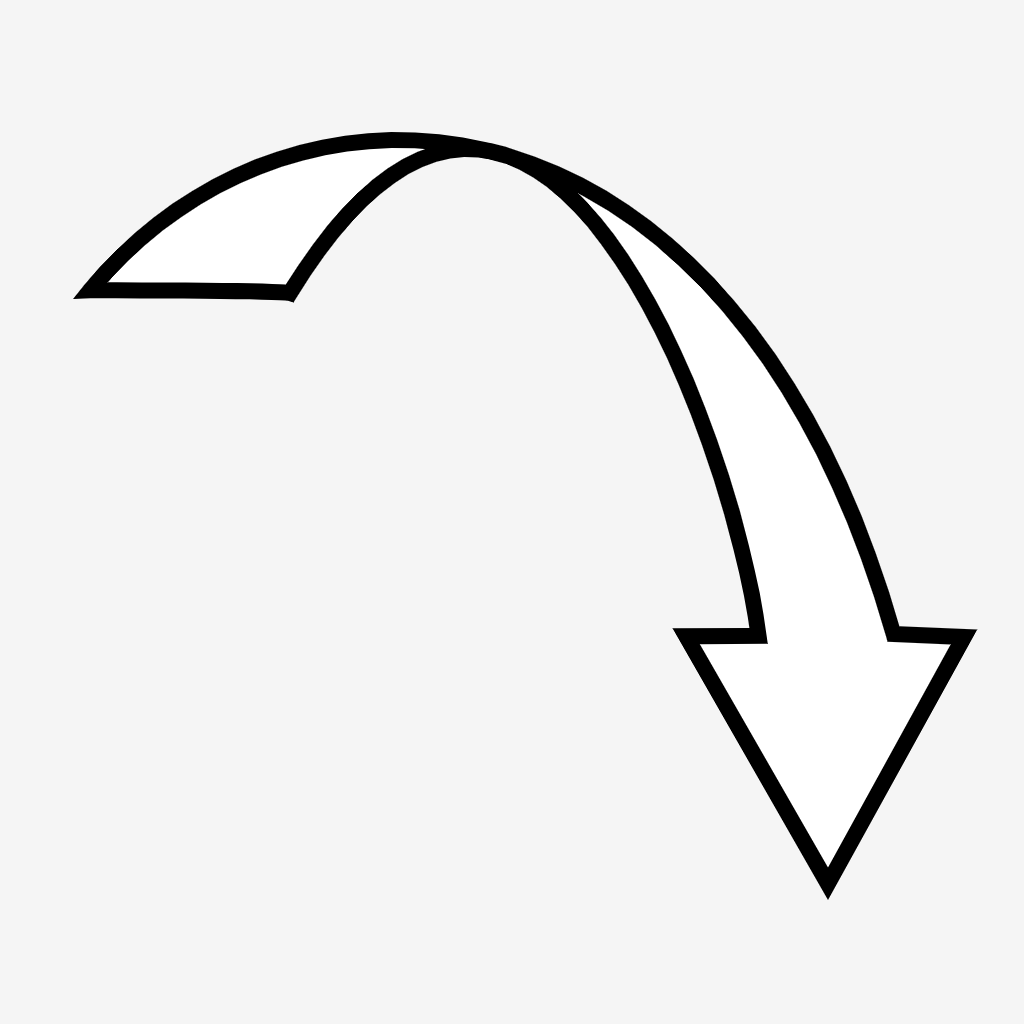
\includegraphics[width=0.75cm]{icons/flip_white.png}
	};
}

\newcommand{\topCollectIncome}{
	\node at (0.5*\cardwidth, 0.7*\cardheight) {
		
\includegraphics[width=2cm]{icons/collect_income.png}
	};
}
\newcommand{\topSpendMoney}[1]{
	\filldraw[red,fill=white!85!red] (0.5*\cardwidth, 0.7*\cardheight) circle (\costcirclesize cm);
	\node[text width=1.5cm] at (0.5*\cardwidth, 0.7*\cardheight+0.5*\costcirclesize) {
		\begin{center}
			\Large \textbf #1
		\end{center}
	};
}
\newcommand{\topGainMoney}[1]{
	\filldraw[green,fill=white!85!green] (0.5*\cardwidth, 0.7*\cardheight) circle (\costcirclesize cm);
	\node[text width=0.5cm] at (0.5*\cardwidth, 0.7*\cardheight+0.5*\costcirclesize+0.35) {
		\begin{center}
			\Large \textbf #1
		\end{center}
	};
}
\newcommand{\topPlayCard}{
	\draw[black,smallcardcorners,fill=black] (0.5*\cardwidth-0.5,0.7*\cardheight-0.75) rectangle (0.5*\cardwidth+0.5,0.7*\cardheight+0.75);
	\node[text width=2cm] at (0.5*\cardwidth, 0.7*\cardheight-0.75) {
		\begin{center}
			
\includegraphics[width=0.75cm]{icons/play_arrow_white.png}
		\end{center}
	};
	\filldraw[red,fill=white!85!red] (0.5*\cardwidth+0.6,0.7*\cardheight+0.75) circle (0.25cm);
	\node[text width=0.25cm] at (0.5*\cardwidth+0.6, 0.7*\cardheight+0.75+0.25) {
		\begin{center}
			\small X
		\end{center}
	};
}


\newcommand{\middlePlaceTile}[2]{
	\node[flathexa,fill=#1] at (0.5*\cardwidth, 0.5*\cardheight-0.5*\hexSize) {
		\includegraphics[width=\hexIconSize cm]{#2}
	};
}
\newcommand{\middleGainAction}{
	\node at (0.5*\cardwidth, 0.5*\cardheight) {
		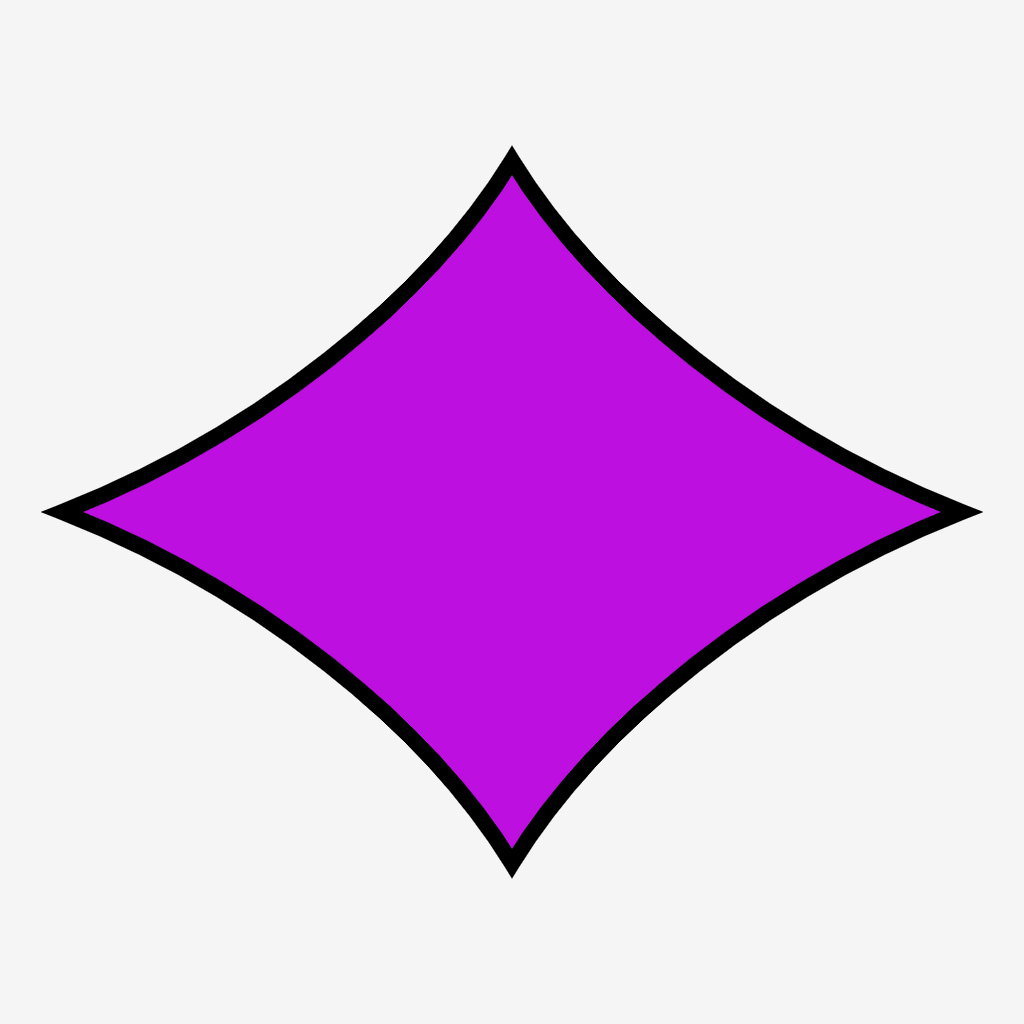
\includegraphics[width=1.5cm,height=3cm]{icons/activation_diamond_purple_189-16-224.png}
	};
}
\newcommand{\middleCollectIncome}{
	\node at (0.5*\cardwidth, 0.5*\cardheight) {
		
\includegraphics[width=2cm]{icons/collect_income.png}
	};
}
\newcommand{\middleAbilityText}[1]{
	\node[text width=\cardwidth cm] at (0.5*\cardwidth, 0.5*\cardheight) {
		\begin{center}
			\large \textbf #1
		\end{center}
	};
}

\newcommand{\middleGainMoney}[1]{
	\filldraw[green,fill=white!85!green] (0.5*\cardwidth, 0.5*\cardheight) circle (\costcirclesize cm);
	\node[text width=1cm] at (0.5*\cardwidth, 0.5*\cardheight+0.5*\costcirclesize) {
		\begin{center}
			\Large \textbf #1
		\end{center}
	};
}

\newcommand{\bottomPlaceTile}[2]{
	\node[flathexa,fill=#1] at (0.5*\cardwidth, 0.3*\cardheight-0.5*\hexSize) {
		\includegraphics[width=\hexIconSize cm]{#2}
	};
}
\newcommand{\bottomDrawCard}{
	\node at (0.5*\cardwidth, 0.3*\cardheight) {
		
\includegraphics[width=2cm]{icons/card_draw.png}
	};
}
\newcommand{\bottomGainMoney}[1]{
	\filldraw[green,fill=white!85!green] (0.5*\cardwidth, 0.3*\cardheight) circle (\costcirclesize cm);
	\node[text width=1cm] at (0.5*\cardwidth, 0.3*\cardheight+0.5*\costcirclesize) {
		\begin{center}
			\Large \textbf #1
		\end{center}
	};
}
\newcommand{\bottomGainAction}{
	\node at (0.5*\cardwidth, 0.3*\cardheight) {
		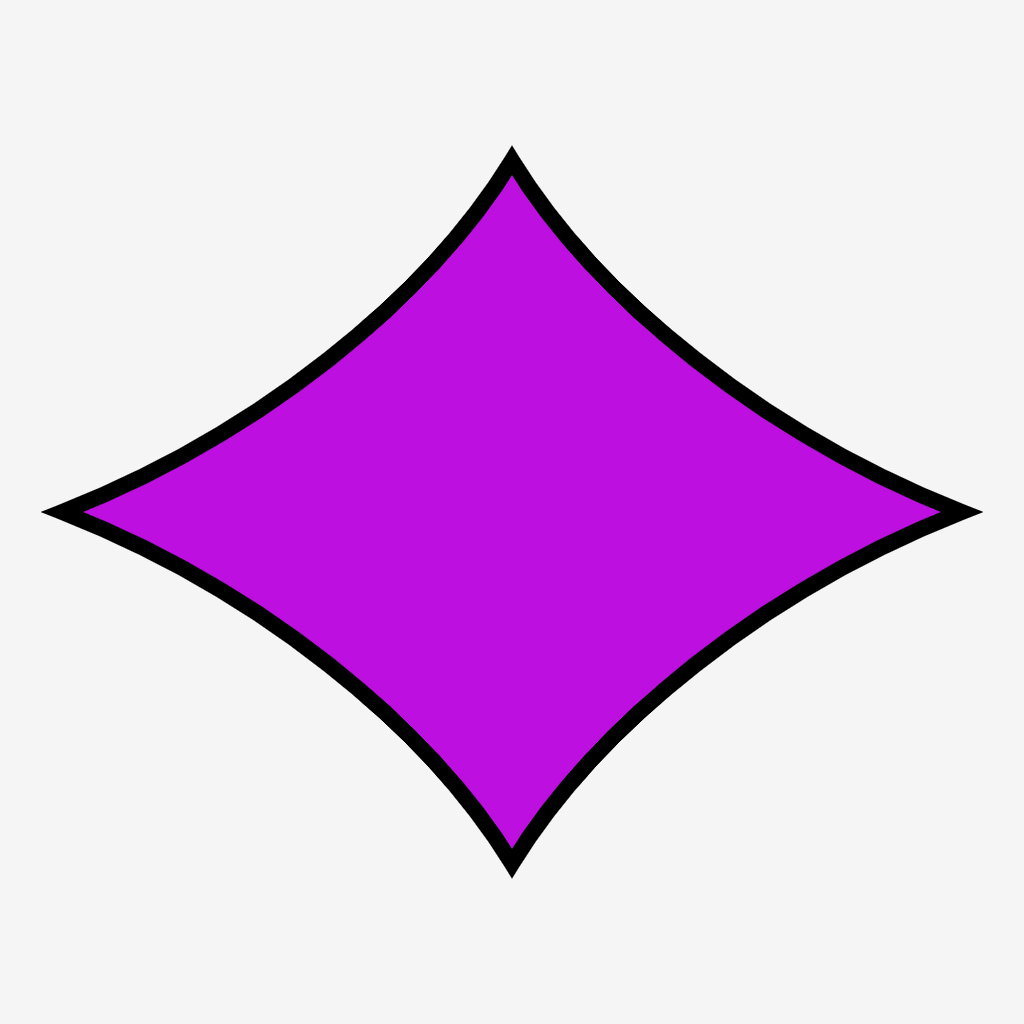
\includegraphics[width=1.5cm,height=3cm]{icons/activation_diamond_purple_189-16-224.png}
	};
}
\newcommand{\bottomTileAndAction}[2]{
	\node[flathexa,fill=#1] at (0.3*\cardwidth, 0.3*\cardheight-0.5*\hexSize) {
		\includegraphics[width=\hexIconSize cm]{#2}
	};
	\node at (0.7*\cardwidth, 0.3*\cardheight) {
		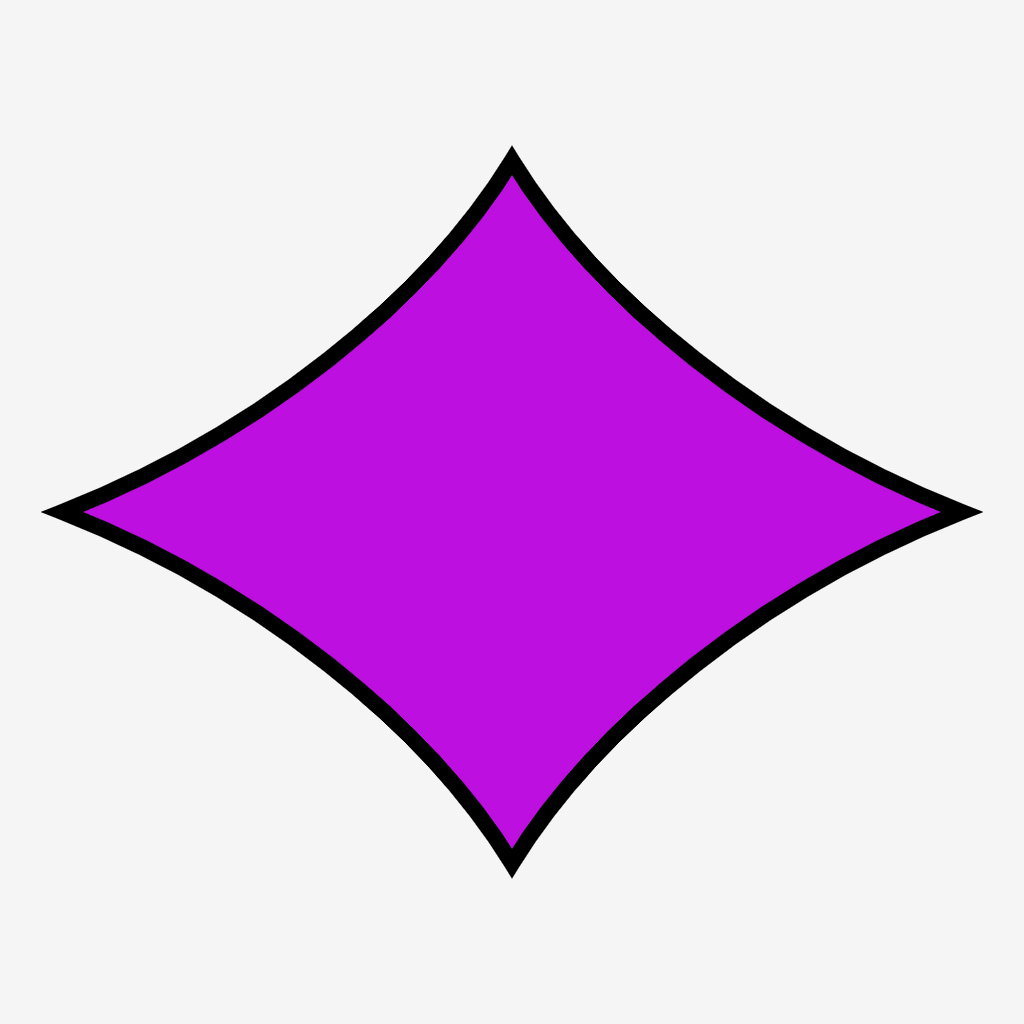
\includegraphics[width=1.5cm,height=3cm]{icons/activation_diamond_purple_189-16-224.png}
	};
}
\newcommand{\bottomCollectIncome}{
	\node at (0.5*\cardwidth, 0.3*\cardheight) {
		
\includegraphics[width=2cm]{icons/collect_income.png}
	};
}
\newcommand{\bottomPlayCard}{
	\draw[black,smallcardcorners,fill=black] (0.5*\cardwidth-0.5,0.3*\cardheight-0.75) rectangle (0.5*\cardwidth+0.5,0.3*\cardheight+0.75);
	\node[text width=2cm] at (0.5*\cardwidth, 0.3*\cardheight-0.75) {
		\begin{center}
			
\includegraphics[width=0.75cm]{icons/play_arrow_white.png}
		\end{center}
	};
	\filldraw[red,fill=white!85!red] (0.5*\cardwidth+0.6,0.3*\cardheight+0.75) circle (0.25cm);
	\node[text width=0.25cm] at (0.5*\cardwidth+0.6, 0.3*\cardheight+0.75+0.25) {
		\begin{center}
			\small X
		\end{center}
	};
}
\newcommand{\bottomTileFlip}{
	\draw[black,smallcardcorners,fill=white] (0.5*\cardwidth-0.6,0.3*\cardheight-0.6) rectangle (0.5*\cardwidth+0.6,0.3*\cardheight+0.6);
	\node at (0.5*\cardwidth+0.4, 0.3*\cardheight-0.2) {
		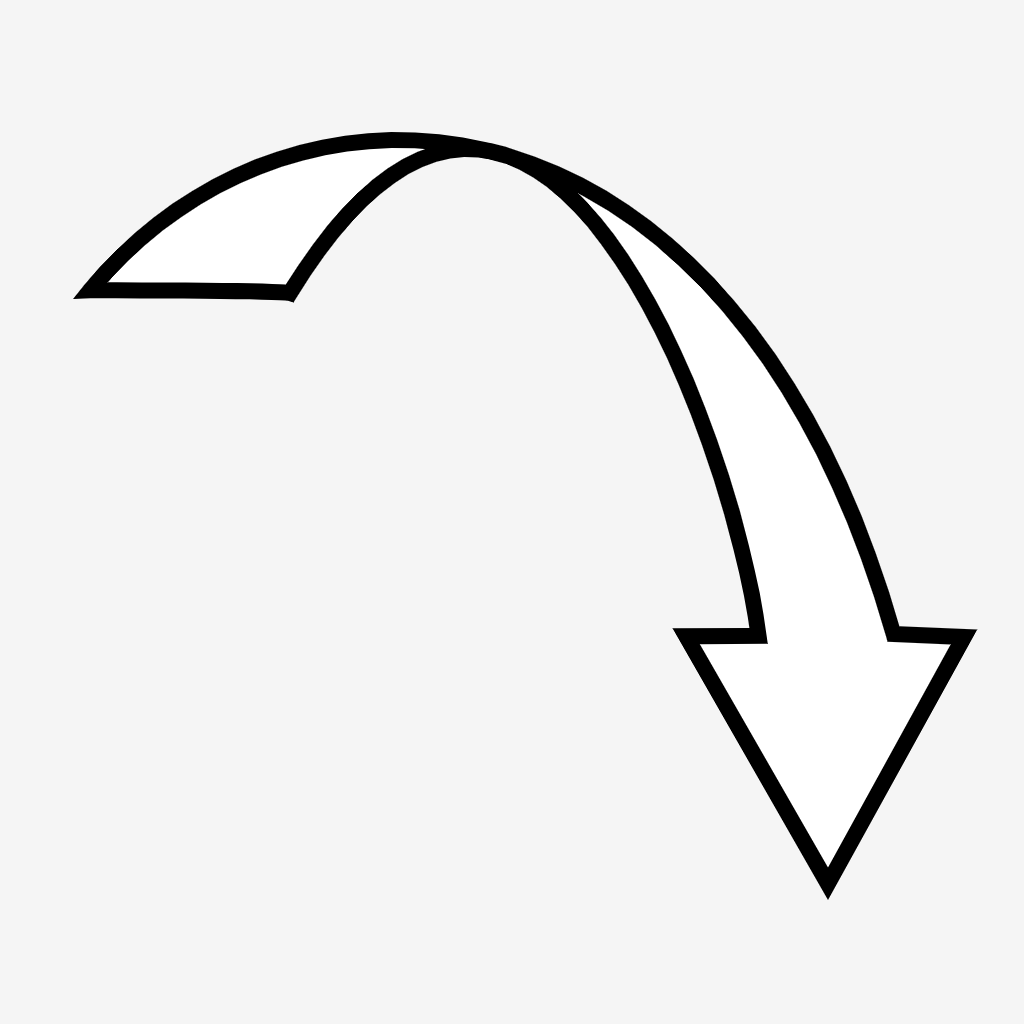
\includegraphics[width=0.75cm]{icons/flip_white.png}
	};
}

\newcommand{\terraformingPoints}[1]{
	\filldraw[green,fill=white!85!green] (0.5*\cardwidth-1, 0.4) rectangle (0.5*\cardwidth+1, 1.1);
	\node[text width=\cardwidth cm] at (0.5*\cardwidth, 0.9) {
		\begin{center}
			\raisebox{0.25cm}{#1}
			
\includegraphics[height=0.7cm]{icons/achievement_white.png}
		\end{center}
	};
}
\newcommand{\terraformingPointsPerTile}[3]{
	\filldraw[green,fill=white!85!green] (0.5*\cardwidth-2, 0.4) rectangle (0.5*\cardwidth+2, 1.1);
	\node[text width=\cardwidth cm] at (0.4*\cardwidth, 0.9) {
		\begin{center}
			\raisebox{0.25cm}{#1}
			
\includegraphics[height=0.7cm]{icons/achievement_white.png}
			\raisebox{0.25cm}{/}
		\end{center}
	};
	\node[tinyhexa,fill=#2] at (0.6*\cardwidth, 0.75-0.5*\tinyhexSize) {
		\includegraphics[width=\tinyhexIconSize cm]{#3}
	};
}

